\chapter{\IfLanguageName{dutch}{Stand van zaken}{State of the art}}
\label{ch:stand-van-zaken}

% Tip: Begin elk hoofdstuk met een paragraaf inleiding die beschrijft hoe
% dit hoofdstuk past binnen het geheel van de bachelorproef. Geef in het
% bijzonder aan wat de link is met het vorige en volgende hoofdstuk.

% Pas na deze inleidende paragraaf komt de eerste sectiehoofding.

\section{Personalisatie}
\label{sec:Personalisatie}

Personalisatie van webapplicaties en websites draait erom de bezoekers een op maat gemaakte ervaring aan te bieden. Dit kan op verschillende manieren toegepast worden, en kan meerdere doelen hebben. In dit hoofdstuk wordt er verder ingegaan op welke manieren personalisatie van websites wordt toegepast, en wat dit betekent voor zowel de bezoeker als het bedrijf zelf.

\subsection{Personalisatie op basis van e-mail en sociale media}
\label{subsec:Personalisatie op basis van e-mail en Social Media}

Zowat iedereen heeft wel te kampen met een overvloed aan e-mails in hun postvak van allerlei websites waar ze hun e-mailadres ooit hebben vrijgegeven. U zou denken dat deze door de meeste mensen simpelweg verwijderd worden, maar e-mailmarketing blijft een van de meest succesvolle marketingstrategieën \autocite{Dehkordi2012}. E-mailmarketing is relatief makkelijk te implementeren en vereist weinig technische investering, meestal wordt dit verwezenlijkt via systemen van derden zoals bijvoorbeeld \href{https://mailchimp.com/}{MailChimp}. Een nadeel van deze marketingvorm is dat het bedrijf continu bezig moet zijn met nieuwe inhoud te creëren voor deze e-mails, alsook op de website waar de marketingmails over gaan. 

\subsection{Personalisatie op basis van geografische locatie}
\label{subsec:Personalisatie op basis van geografische locatie}

Geografische personalisatie is het aanpassen van de website op basis van de locatie van de gebruiker. Gebruikers uit België die naar de website van een internationaal bedrijf surfen, zullen dan worden omgeleid naar een Nederlandse of Franse versie van die website.

Geografische personalisatie kan ook gebruikt worden om de inhoud van een pagina aan te passen aan de hand van de locatie van de gebruiker, of om vertalingen aan te bieden.
Een nadeel hiervan is dat mensen die op reis gaan het soms moeilijk zouden kunnen hebben om naar de juiste versie van de website te navigeren, aangezien het systeem de gebruiker zal willen omleiden naar de pagina of inhoud die voorzien is voor het land waar zij zich momenteel in bevinden. Eenzelfde probleem kan zich voordoen bij bedrijven die hun webverkeer omleiden via een ander land door middel van bijvoorbeeld een VPN. 

Geografische personalisatie is ook relatief eenvoudig te implementeren en kan een grote troef zijn op de internationale markt. 

\subsection{Personalisatie op basis van IP-adres}
\label{subsec:Personalisatie op basis van IP-adres}

Deze methode van personalisatie is wat minder opvallend, aangezien het bij de gemiddelde internetgebruiker weinig tot nooit zal voorkomen, aangezien zij het internet gebruiken via een serviceprovider zoals Telenet of Proximus. 

Deze vorm van personalisatie wordt gebruikt om zakelijke gebruikers en bedrijven te kunnen identificeren op basis van hun IP-adres. Zo kan men zien of een bezoeker bij een bepaald bedrijf werkzaam is om deze direct aan te spreken op bijvoorbeeld de homepagina.

	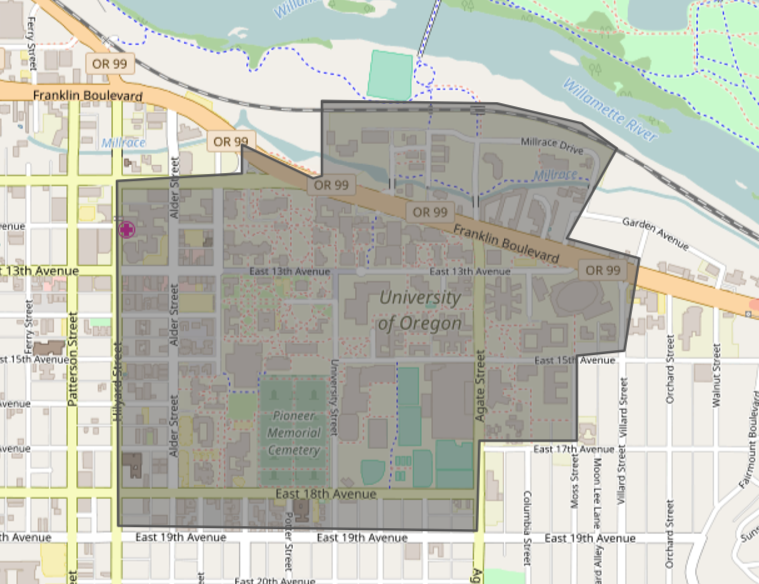
\includegraphics[width=\linewidth]{img/e2fcfe784532c41a644e4465f535530d}

Net zoals bij personalisatie op basis van locatie kan dit misleidende resultaten opleveren, bijvoorbeeld als de werknemer van thuis werkt of het IP-adres niet duidelijk aantoont vanuit welk bedrijf het webverkeer van de bezoeker afkomstig is. Ook voor performantie kan dit negatieve gevolgen hebben, aangezien deze vorm van personalisatie afhankelijk is van systemen van derden. 

Verder moet er ook inhoud gecreëerd worden voor elk bedrijf dat men specifiek wil aanspreken. Dit is een tijdrovend proces, maar aangezien deze vorm van personalisatie weinig voorkomt, is het wel een troef waardoor het bedrijf zich kan onderscheiden van de meerderheid en zich kan laten opvallen.

  
 \subsection{Verwante inhoud personalisatie}
 \label{subsec:Verwante inhoud personalisatie}
 
 Dit is de vorm van personalisatie die een grote meerwaarde zal leveren aan dit onderzoek. De meeste mensen hebben deze vorm al ondervonden op een webshop zoals Amazon of Bol.com. Deze vorm draait erom de gebruikers artikels aan te raden op basis van artikels of inhoud die ze al eerder bekeken hebben, alsook het gedrag van andere gebruikers.
 
De werking van het aanbevelingssysteem van Amazon is gebaseerd op enkele complexe algoritmen  \autocite{Linden2003}. Dit is natuurlijk verantwoord omdat zij op zeer grote schaal werken en veel geld hebben geïnvesteerd in de ontwikkeling van hun systeem. 

In de realiteit hoeven de technologieën voor aanbevelingen van producten niet zo complex te zijn voor gewone webshops en bedrijven, vaak is het voldoende om relaties te creëren tussen artikels en op basis van deze relaties nieuwe artikels aan te raden aan de gebruikers. 

Een voorbeeld van een relatie tussen twee artikels is de welbekende 'Anderen bekeken ook' blok die vaak zichtbaar is bij het bekijken van een detailpagina van een product. 
Een simpelere methode van dergelijke relaties is het aanbieden van verwante producten op basis van categorieën of tags. Tags zijn een manier om kenmerken van een product weer te geven die specifieker zijn dan een categorie. Een categorie kan dan 'schoenen' zijn, terwijl een tag 'lage sneakers' is. 


\section{Wat is Graph?}
\label{sec:wat is Graph?}

In de context van deze bachelorproef zal er met 'Graph' steeds verwezen worden naar een Graph databank. In dit onderdeel zullen we wat dieper ingaan op wat dit soort databank precies inhoudt om een volledig begrijpen van de precieze werking te verzekeren. 

\subsection{SQL}
\label{sec:SQL}
SQL is de afkorting voor Structured Query Language. Dit verwijst eigenlijk naar de programmeertaal die gebruikt wordt om data op te halen of te schrijven naar een databank. Met een SQL-databank wordt dus eigenlijk een relationele databank bedoeld. 
Deze databankstructuur is relationeel opgebouwd, dit wil zeggen dat we gebruik maken van een schema waarin een aantal tabellen met onderlinge relaties staan die gevuld worden door attributen. 

	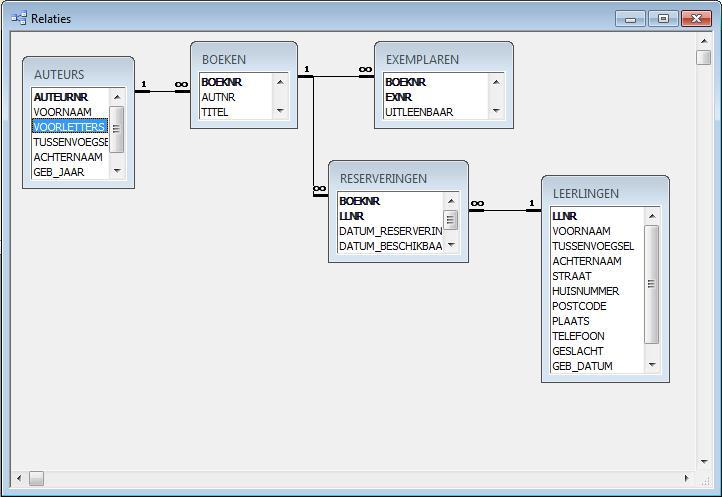
\includegraphics[width=\linewidth]{img/3-0.jpg}
	
Bovenstaande figuur is een voorbeeld van dergelijk schema, de relaties tussen te tabellen zijn eenvoudig af te leiden aan de hand van de lijnen.

Het opvragen van data gebeurt aan de hand van query's, letterlijk vertaald uit het Engels betekent dit 'vraag'. Een query wordt bijvoorbeeld als volgt opgebouwd: 

SELECT name 
FROM boeken b
JOIN auteurs a
WHERE b.auteurnummer = a.nummer
ORDER BY titel

Deze query zal een lijst van namen van alle boeken in de databank van een bepaalde auteur weergeven, gesorteerd op titel.

Merk hierbij op dat we het woord  'JOIN' gebruiken om aan het systeem duidelijk te maken dat we de data uit zowel de tabel 'boeken' als de tabel 'auteurs' nodig hebben. Dit is handig op kleine schaal, maar wanneer we data uit een groot aantal verschillende tabellen nodig hebben, kunnen deze query's zeer complex en traag worden. Dit soort scenario's is waar NoSQL uitblinkt.


\subsection{NoSQL}
\label{sec:NoSQL}
Graph is een NoSQL databank. een NoSQL databank laat toe tot het opslaan en ophalen van data via een model dat de limitaties van relationele (SQL) databanken zoals hierboven besproken overbrugt. 
Het grote verschil hierbij is dat NoSQL databanksystemen niet altijd vaste schema's volgen, er hoeft dus niet op voorhand gedefinieerd te worden hoe de data gestructureerd zal zijn, en er hoeven dus bijgevolg ook geen relaties gedefinieerd te worden, dit systeem is dus veel flexibeler. 


	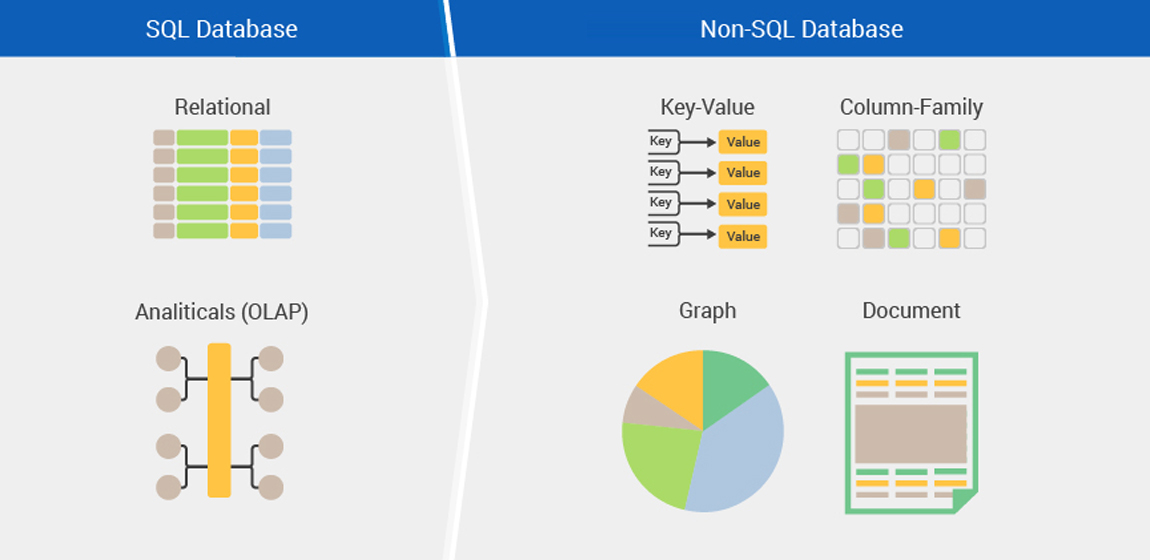
\includegraphics[width=\linewidth]{img/5_things_you_must_consider_before_nosql1.jpg}
	
NoSQL maakt gebruik van diverse opslagmethodes, enkele veelvoorkomende methodes worden hieronder verder uitgelegd. 


\subsubsection{Document}
\label{sec:Document}

Bij een Document store //REF wordt data opgeslagen op een semi-gestructureerde wijze. Ze laten toe dat er verschillende types documenten binnen dezelfde opslag mogelijk zijn, dat er bepaalde velden optioneel zijn of een ander coderingssysteem gebruiken.

	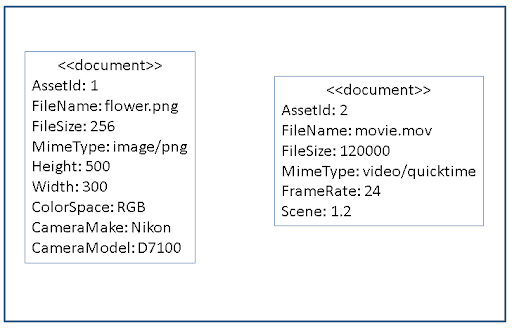
\includegraphics[width=\linewidth]{img/documentStoreExample.png}
	
\subsubsection{Key-Value}
\label{sec:Key-Value}

Deze opslagmethode is vooral geschikt wanneer data vaak uitgelezen moet worden. Het idee hiervan is hetzelfde als een Hashmap, waarbij een functie een sleutel omzet in een hash-waarde om die key-value combinatie snel te kunnen vinden. Dit wordt in onderstaande figuur geïllustreerd. Doordat de data enkel via deze waarde te vinden is, kan deze in een constante tijd worden opgehaald. Deze structuur blinkt dus uit in gevallen waarbij er zeer veel data is om te doorzoeken.

	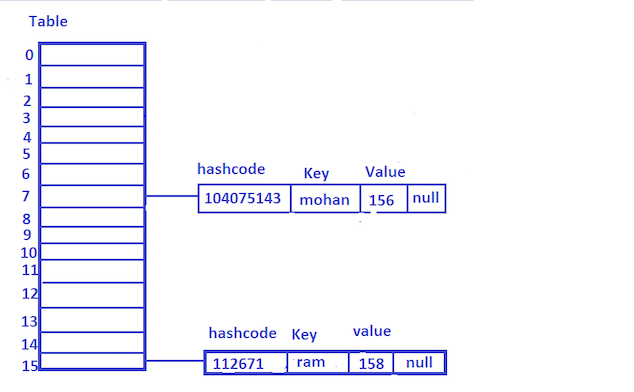
\includegraphics[width=\linewidth]{img/hashMapExample.png}

\subsubsection{Graph}
\label{sec:Graph}

Dit is de structuur die verder in dit onderzoek gebruikt zal worden. Deze structuur maakt gebruik van een wiskundige graaf om data op te slaan. Een graaf bestaat uit een aantal knopen (genaamd nodes) die al dan niet verbonden zijn. Een groot voordeel hiervan is dat deze databanken sneller zijn dan relationele databanken omdat ze snel naar een bepaalde node kunnen verwijzen, waarbij we bij een relationele databank een JOIN zouden moeten gebruiken. 

	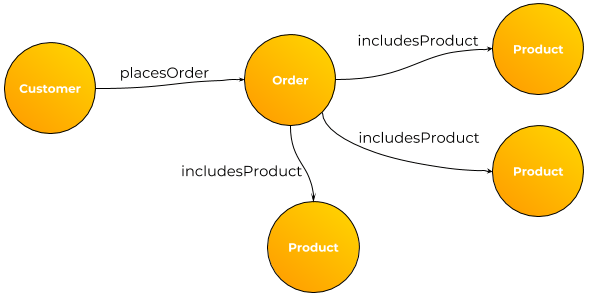
\includegraphics[width=\linewidth]{img/Customer-Order-Example-Graph.png}
	
\subsection{Neo4j}
\label{sec:Neo4j}

Er bestaan verschillende platformen voor SQL, alsook verschillende platformen voor de hierboven beschreven NoSQL databanken. Neo4j is een van de meer bekende platformen voor graph databanken, dit platform zal gebruikt worden in dit onderzoek.

Walmart maakt gebruik van Neo4j om de aanbevelingen voor hun klanten op hun online webservices te optimaliseren \autocite{neo4jWalmart2014}. Zij gebruiken dit omdat graph databanken zeer snel over een gebruiker zijn koophistorie kunnen traverseren, en ook direct nieuwe mogelijke interesses kunnen halen uit het gedrag van de gebruiker. Daarmee wordt bedoeld dat er in real-time nieuwe connecties worden gelegd tussen de gebruiker en de producten, en hij de nieuwe aanbevelingen meteen zal zien, en niet enkele dagen of uren later. Er wordt dus historische data gematcht met real-time data, hier blinkt Neo4j in uit. 


% TODO: Info van hieruit gebruiken en bronnen vermelden (zie pdf's van use cases)
% https://bbvaopen4u.com/en/actualidad/neo4j-what-graph-database-and-what-it-used


\section{Wat is ElasticSearch?}
\label{sec:wat is ElasticSearch?}

Elasticsearch op zichzelf is eigenlijk een zoekmachine die data kan analyseren, of dit nu nummers, tekst, gestructureerd of ongestructureerd is. Elasticsearch is een component van de Elastic stack, ook wel ELK-Stack genoemd. Dit staat voor Elasticsearch, Logstash en Kibana. Logstash wordt gebruikt om data te verwerken uit meerdere bronnen en te versturen naar Elasticsearch. Kibana is een tool om de gebruikers een visueel beeld te geven van de data in de vorm van grafieken of tabellen.

In Elasticsearch is het mogelijk gewichten toe te kennen aan de resultaten van een zoekopdracht, zo kunnen meer relevante resultaten hoger in de lijst staan, dit is een belangrijke factor in dit onderzoek, namelijk of deze technologie gebruikt kan worden in E-Commerce toepassingen. In het artikel van \cite{Vavliakis2019} wordt beweerd dat het systeem dat zij implementeerden op een performante manier de gewenste resultaten gaf, alsook dat dit een oplossing kan zijn voor real-time zoekopdrachten in commerciële toepassingen.
